\documentclass[usenames,dvipsnames,aspectratio=1610]{beamer}

%\setbeamertemplate{nagivation symbols}{}
%%% Standard includes
\usepackage{amsthm, amssymb, amsmath, hyperref}
\usepackage{subfig,multicol}

\usepackage[T1]{fontenc}
\usepackage{lmodern}

\usetheme[sectionpage=none]{metropolis}
\setbeamertemplate{subsection in toc}[sections numbered]

%%% Graphics 
%\usepackage{tikz}
\usepackage{tikz-cd}
\usetikzlibrary{positioning, calc}
\usetikzlibrary{matrix,arrows,decorations.pathmorphing}
\usetikzlibrary{shapes,arrows.meta,decorations.markings}
%\usepackage[all]{xy}
%\usepackage{graphicx}
%\usepackage{subcaption}


%%% Margins, formatting
%\usepackage{fullpage}
%\usepackage[margin=1in]{geometry}
\usepackage{setspace}
\usepackage{fancyhdr,lastpage}
%\usepackage{afterpage}
%\pagenumbering{gobble}
%\addtolength{\textwidth}{4cm}
%\addtolength{\hoffset}{-2cm}
%\addtolength{\textheight}{3.5cm}
%\addtolength{\voffset}{-2.5cm}
%\fancyhead{}
%\doublespacing
%\usepackage{enumitem} %%enumitem is incompatible with beamer
%\setitemize{noitemsep}
%\linespacing{1.1em}


%% Define the headers and footers for the first page, call it 'first'
%\fancypagestyle{first}{%
  %\renewcommand{\headrulewidth}{0pt}
%\fancyfoot[C]{\thepage~of~\pageref{LastPage}}
%\renewcommand{\footrulewidth}{0pt}}

%\usepackage{multicol}

%%% Bibliography
\usepackage[
backend=bibtex,
style=numeric,
block=space
]{biblatex}
\addbibresource{ref1.bib}
\renewbibmacro{in:}{}
\DeclareNameAlias{sortname}{first-last}

%%% Fonts
%\usepackage{helvet}
%\usepackage{anyfontsize,libertine}
%\usepackage{libertinust1math}
%\usepackage[T1]{fontenc}
%\usepackage{mathpazo}
%\usepackage{eulervm}
%\renewcommand{\familydefault}{\sfdefault}


% Quiet beamer complaints
\renewcommand\textbullet{\ensuremath{\bullet}}



%%% New commands

\newcommand{\Mdef}[2]{\newcommand{#1}{\relax \ifmmode #2 \else $#2$\fi}}

%% thereoms, prop, etc
%\newtheorem{theorem}{Theorem}
%\newtheorem{lemma}[theorem]{Lemma}
%\newtheorem{prop}[theorem]{Proposition}
%\newtheorem{definition}[theorem]{Definition}
%\newtheorem{corollary}[theorem]{Corollary}
%\newtheorem{example}[theorem]{Example}
%\newtheorem{remark}[theorem]{Remark}
%\newtheorem{conjecture}[theorem]{Conjecture}
%\newtheorem*{question}{Question}
%\newtheorem*{questions}{Questions}

%% operators
\DeclareMathOperator{\Hom}{Hom}
\DeclareMathOperator{\cok}{cok}
\DeclareMathOperator{\im}{im}
\DeclareMathOperator{\id}{id}

%% Letters
\Mdef{\SA}{\mathcal{A}}
\Mdef{\SAD}{\mathcal{A}_*}
\Mdef{\SAS}{\mathrm{Sq}}
\Mdef{\SAP}{\mathcal{P}}

\Mdef{\B}{B}
\Mdef{\F}{\mathbb{F}}
\Mdef{\M}{\mathcal{M}}
\Mdef{\N}{\mathbb{N}}
\Mdef{\R}{\mathbb{R}}
\Mdef{\Z}{\mathbb{Z}}
\Mdef{\Q}{\mathbb{Q}}
\Mdef{\vectk}{\mathrm{vect}_k}

\newcommand{\Fp}[1]{\mathbb{F}_{#1}}
\newcommand{\HPM}[1]{H_{#1}^{\mathrm{MP}}(f;\mathbb{F}_2)}


%% arrows
\newcommand{\ra}{\rightarrow}
\newcommand{\lra}{\longrightarrow}
\newcommand{\la}{\leftarrow}
\newcommand{\lla}{\longleftarrow}

%% symbols
\newcommand{\tensor}{\otimes}
\newcommand{\dsum}{\oplus}
\newcommand{\Dsum}{\bigoplus}
\newcommand{\susp}{\Sigma}



\tikzstyle{decision} = [diamond, draw, fill=blue!20, 
    text width=4.5em, text badly centered, node distance=3cm, inner sep=0pt]
\tikzstyle{block} = [rectangle, draw, fill=blue!20, 
    text width=5em, text centered, rounded corners, minimum height=4em]
\tikzstyle{wideblock} = [rectangle, draw, fill=blue!20, 
    text width=7em, text centered, rounded corners, minimum height=4em]
%\tikzstyle{line} = [draw, -latex']
\tikzstyle{line} = [draw, -Latex]
\tikzstyle{cloud} = [draw, ellipse,fill=red!20, node distance=3cm,
    minimum height=2em]
%%%%%%%%%%%%%%%%%%%%%%%%

%======================================================================

\title{An Introduction to Topological Data Analysis}
\author{Matthew Zabka}
\date{Laber Labs \\ North Carolina State University}
\institute{Southwest Minnesota State University}

\begin{document}
\setbeamercolor{background canvas}{bg=white}
\begin{frame}[plain]
  \maketitle
\end{frame}

\metroset{block=fill}

\begin{frame}{Outline}
  \tableofcontents
\end{frame}

%===========================================================================

\section{Crash course in algebraic topology}
\begin{frame}
  \frametitle{Algebraic Topology}
  \begin{block}{What is algebraic topology?}
    Topology is a branch of mathematics which is good at extracting global
    qualitative features from complicated geometric structures. 
    
    Algebraic topology provides a set of {\em algebraic} descriptors to topological objects.
  \end{block}
  \pause

  \begin{block}{Questions and scope}
    Topological questions surround different notions of connectedness:
    connected components, loops, voids, etc.

    Two topological spaces are equivalent through the lens of topology if one
    can be {\em continuously} deformed to the other. 
  \end{block}
  \center{\fontsize{40}{40}\selectfont \textsf{A B C D}}
\end{frame}
%---------------------------------------------------------

\begin{frame}
  \frametitle{Algebraic Topology}
  \begin{block}{What is algebraic topology?}
    Topology is a branch of mathematics which is good at extracting global
    qualitative features from complicated geometric structures. 
    
    Algebraic topology provides a set of {\em algebraic} descriptors to topological objects.
  \end{block}

  \begin{block}{Questions and scope}
    Topological questions surround different notions of connectedness:
    connected components, loops, voids, etc.

    Two topological spaces are equivalent through the lens of topology if one
    can be {\em continuously} deformed to the other. 
  \end{block}
  \center{\fontsize{40}{40}\selectfont \textsf{ {\color{red} A} B C {\color{red} {D}}}}
\end{frame}

%-------------------------------------------------------------------------------------------

\begin{frame}{Invariants of topological spaces}
  \begin{itemize}
    \item Algebraic Topology assigns {\em invariants} to topological spaces.
      These take the form of groups, rings, fields, vector spaces, etc.
    \item Our computations will be over the field $\F_2$, so it suffices to record
      only the {\em dimensions} of vector spaces. 
    \item If two spaces are the same, then the invariants must be the same. 
      
      If the invariants are not the same, then the two spaces are not the same.
  \end{itemize}
\end{frame}

%================================================================================

\section{Persistent Homology and examples}
\begin{frame}{Topological Data Analysis}
  \begin{alertblock}{Goal}
    {\bf Topological data analysis uses topology to summarize and study the
    `shape' of data.}
  \end{alertblock}
  \vspace{-0.1in}
  \pause
  Examples:
  \vspace{-0.1in}
  \begin{itemize}
  \begin{multicols}{2}
  \item motion tracking problems,
  \item analysis of brain arteries,
  \item analysis of social and spatial networks, including neuronal
    networks, Twitter, co-authorship,
  \item study of viral evolution,
  \item measurement of protein compressibility,
  \item analysis of phase transitions,
  \item financial crash analysis,
  \item piecewise constant signal analysis,
  \item study of cosmic web and its filamentary structure,
  \item identification of breast cancer subtypes,
  \item study of plant root systems,
  \item discrimination of EEG signals before and during epileptic seizures,
  \item steganalysis of images,
  \item sphere packings,
  \item population activity in the visual cortex,
  \item fMRI data
  \end{multicols}

  \end{itemize}
\end{frame}

%--------------------------------------------------------------------------------

\begin{frame}{Overview of TDA}
  Topological data analysis comes in a variety of flavors. 
  
  The two most popular methods in TDA are
  \begin{center}
    1. Persistent Homology \\
    2.  Mapper
  \end{center}
\end{frame}

%------------------------------------------------------------------------

\begin{frame}
  \frametitle{Simplicial Complexes}
  A {\em simplicial complex} is a combinatorial object, generalizing the notion of a graph. Each
  simplicial complex is built out of {\em simplices} of varying dimensions.

  \begin{center}
    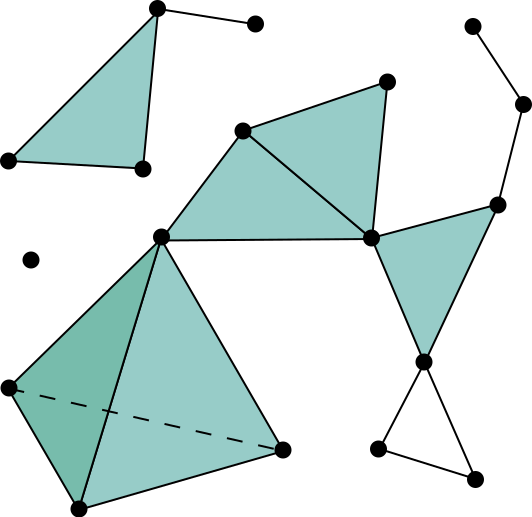
\includegraphics[scale=0.35]{images/Simplicial_complex_example.png}
  \end{center}
\end{frame}

%------------------------------------------------------------------------

\begin{frame}
  \frametitle{Betti numbers of simplicial complexes}
  \begin{align*}
    \beta_0 & =  \# \text{ of connected components}\\
    \beta_1 & =  \# \text{ of holes}\\
    \beta_2 & =  \# \text{ of voids}
  \end{align*}
  \begin{columns}
    \begin{column}{0.4\textwidth}
      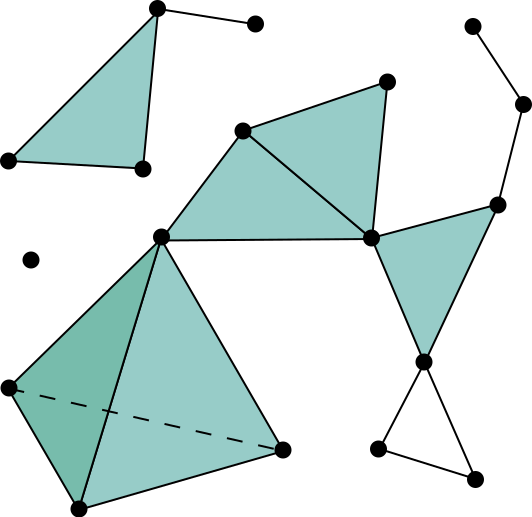
\includegraphics[height=45mm]{images/Simplicial_complex_example.png}
    \end{column}
    \begin{column}{0.2\textwidth}
      \begin{eqnarray*}
        \beta_0 & = & \visible<2>{3}\\
        \beta_1 & = & \visible<2>{1}\\
        \beta_2 & = & \visible<2>{1}
      \end{eqnarray*}
    \end{column}
  \end{columns}
  \bigskip
\end{frame}

%------------------------------------------------------------------------

\begin{frame} \frametitle{Homology of simplicial complexes}
  \begin{definition}
    Homology in degree $k$ is given by $k$-cycles modulo the $k$-boundaries.
  \end{definition}

\begin{center}
\definecolor{zzttqq}{rgb}{0.6,0.2,0}
\definecolor{qqqqff}{rgb}{0,0,1}
\begin{tikzpicture}[line cap=round,line join=round,x=1.0cm,y=1.0cm,scale=1.5]
% \draw[->,color=black] (-4.3,0) -- (7.5,0);
% \foreach \x in {-4,-3,-2,-1,1,2,3,4,5,6,7}
% \draw[shift={(\x,0)},color=black] (0pt,2pt) -- (0pt,-2pt) node[below] {\footnotesize $\x$};
% \draw[->,color=black] (0,-3.1) -- (0,6.3);
% \foreach \y in {-3,-2,-1,1,2,3,4,5,6}
% \draw[shift={(0,\y)},color=black] (2pt,0pt) -- (-2pt,0pt) node[left] {\footnotesize $\y$};
% \draw[color=black] (0pt,-10pt) node[right] {\footnotesize $0$};
% \clip(-4.3,-3.1) rectangle (7.5,6.3);
\fill[color=red,fill=red,fill opacity=0.2] (1,4.5) -- (2.1,5.3) -- (2.4,4.1) -- cycle;
\fill[color=red,fill=red,fill opacity=0.2] (1,4.5) -- (1,3) -- (2.4,4.1) -- cycle;
\fill[color=red,fill=red,fill opacity=0.2] (1,3) -- (1.8,2.2) -- (2.4,4.1) -- cycle;
\fill[color=red,fill=red,fill opacity=0.2] (1.8,2.2) -- (2.5,2.9) -- (2.4,4.1) -- cycle;
\fill[color=red,fill=red,fill opacity=0.2] (2.1,5.3) -- (3.7,4.9) -- (2.4,4.1) -- cycle;
\fill[color=red,fill=red,fill opacity=0.2] (3.7,4.9) -- (2.5,2.9) -- (2.4,4.1) -- cycle;
\fill[color=red,fill=red,fill opacity=0.2] (1.8,2.2) -- (3.1,2.2) -- (2.5,2.9) -- cycle;
\fill[color=red,fill=red,fill opacity=0.2] (3.1,2.2) -- (4,3) -- (5,2.3) -- cycle;
\fill[color=red,fill=red,fill opacity=0.2] (4,3) -- (4.8,3.2) -- (5,2.3) -- cycle;
\fill[color=red,fill=red,fill opacity=0.2] (5.5,4.7) -- (6.2,5.2) -- (6.3,3.9) -- cycle;
\fill[color=red,fill=red,fill opacity=0.2] (6.3,3.9) -- (6.2,2.8) -- (6.9,3.2) -- cycle;
\fill[color=red,fill=red,fill opacity=0.2] (3.7,4.9) -- (4.7,4.5) -- (4,3) -- cycle;
\fill[color=red,fill=red,fill opacity=0.2] (3.7,4.9) -- (5.5,4.7) -- (4.7,4.5) -- cycle;
\fill[color=red,fill=red,fill opacity=0.2] (4.7,4.5) -- (4.8,3.2) -- (4,3) -- cycle;
\fill[color=red,fill=red,fill opacity=0.2] (3.7,4.9) -- (3.4,3.5) -- (2.5,2.9) -- cycle;
\fill[color=red,fill=red,fill opacity=0.2] (3.7,4.9) -- (4,3) -- (3.4,3.5) -- cycle;
\fill[color=red,fill=red,fill opacity=0.2] (2.5,2.9) -- (3.2,2.9) -- (3.4,3.5) -- cycle;
\fill[color=red,fill=red,fill opacity=0.2] (3.2,2.9) -- (3.1,2.2) -- (2.5,2.9) -- cycle;
\fill[color=red,fill=red,fill opacity=0.2] (3.2,2.9) -- (4,3) -- (3.4,3.5) -- cycle;
\fill[color=red,fill=red,fill opacity=0.2] (3.2,2.9) -- (3.1,2.2) -- (4,3) -- cycle;
\draw [thick,color=red] (1,4.5)-- (2.1,5.3);
\draw [thick,color=red] (2.1,5.3)-- (2.4,4.1);
\draw [thick,color=red] (2.4,4.1)-- (1,4.5);
\draw [thick,color=red] (1,4.5)-- (1,3);
\draw [thick,color=red] (1,3)-- (2.4,4.1);
\draw [thick,color=red] (2.4,4.1)-- (1,4.5);
\draw [thick,color=red] (1,3)-- (1.8,2.2);
\draw [thick,color=red] (1.8,2.2)-- (2.4,4.1);
\draw [thick,color=red] (2.4,4.1)-- (1,3);
\draw [thick,color=red] (1.8,2.2)-- (2.5,2.9);
\draw [thick,color=red] (2.5,2.9)-- (2.4,4.1);
\draw [thick,color=red] (2.4,4.1)-- (1.8,2.2);
\draw [thick,color=red] (2.1,5.3)-- (3.7,4.9);
\draw [thick,color=red] (3.7,4.9)-- (2.4,4.1);
\draw [thick,color=red] (2.4,4.1)-- (2.1,5.3);
\draw [thick,color=red] (3.7,4.9)-- (2.5,2.9);
\draw [thick,color=red] (2.5,2.9)-- (2.4,4.1);
\draw [thick,color=red] (2.4,4.1)-- (3.7,4.9);
\draw [thick,color=red] (1.8,2.2)-- (3.1,2.2);
\draw [thick,color=red] (3.1,2.2)-- (2.5,2.9);
\draw [thick,color=red] (2.5,2.9)-- (1.8,2.2);
\draw [thick,color=red] (3.7,4.9)-- (4.7,4.5);
\draw [thick,color=red] (4.7,4.5)-- (5.5,4.7);
\draw [thick,color=red] (3.1,2.2)-- (4,3);
\draw [thick,color=red] (4,3)-- (5,2.3);
\draw [thick,color=red] (5,2.3)-- (3.1,2.2);
\draw [thick,color=red] (4,3)-- (4.8,3.2);
\draw [thick,color=red] (4.8,3.2)-- (5,2.3);
\draw [thick,color=red] (5,2.3)-- (4,3);
\draw [thick,color=red] (5.5,4.7)-- (6.2,5.2);
\draw [thick,color=red] (6.2,5.2)-- (6.3,3.9);
\draw [thick,color=red] (6.3,3.9)-- (5.5,4.7);
\draw [thick,color=red] (6.3,3.9)-- (6.2,2.8);
\draw [thick,color=red] (6.2,2.8)-- (6.9,3.2);
\draw [thick,color=red] (6.9,3.2)-- (6.3,3.9);
\draw [thick,color=red] (5,2.3)-- (6.2,2.8);
\draw [thick,color=red] (3.7,4.9)-- (4.7,4.5);
\draw [thick,color=red] (4.7,4.5)-- (4,3);
\draw [thick,color=red] (4,3)-- (3.7,4.9);
\draw [thick,color=red] (3.7,4.9)-- (5.5,4.7);
\draw [thick,color=red] (5.5,4.7)-- (4.7,4.5);
\draw [thick,color=red] (4.7,4.5)-- (3.7,4.9);
\draw [thick,color=red] (4.7,4.5)-- (4.8,3.2);
\draw [thick,color=red] (4.8,3.2)-- (4,3);
\draw [thick,color=red] (4,3)-- (4.7,4.5);
\draw [thick,color=red] (3.7,4.9)-- (3.4,3.5);
\draw [thick,color=red] (3.4,3.5)-- (2.5,2.9);
\draw [thick,color=red] (2.5,2.9)-- (3.7,4.9);
\draw [thick,color=red] (3.7,4.9)-- (4,3);
\draw [thick,color=red] (4,3)-- (3.4,3.5);
\draw [thick,color=red] (3.4,3.5)-- (3.7,4.9);
\draw [thick,color=red] (2.5,2.9)-- (3.2,2.9);
\draw [thick,color=red] (3.2,2.9)-- (3.4,3.5);
\draw [thick,color=red] (3.4,3.5)-- (2.5,2.9);
\draw [thick,color=red] (3.2,2.9)-- (3.1,2.2);
\draw [thick,color=red] (3.1,2.2)-- (2.5,2.9);
\draw [thick,color=red] (2.5,2.9)-- (3.2,2.9);
\draw [thick,color=red] (3.2,2.9)-- (4,3);
\draw [thick,color=red] (4,3)-- (3.4,3.5);
\draw [thick,color=red] (3.4,3.5)-- (3.2,2.9);
\draw [thick,color=red] (3.2,2.9)-- (3.1,2.2);
\draw [thick,color=red] (3.1,2.2)-- (4,3);
\draw [thick,color=red] (4,3)-- (3.2,2.9);
\begin{scriptsize}
\fill [color=qqqqff] (1,4.5) circle (1.5pt);
\fill [color=qqqqff] (2.1,5.3) circle (1.5pt);
\fill [color=qqqqff] (2.4,4.1) circle (1.5pt);
\fill [color=qqqqff] (1,3) circle (1.5pt);
\fill [color=qqqqff] (1.8,2.2) circle (1.5pt);
\fill [color=qqqqff] (2.5,2.9) circle (1.5pt);
\fill [color=qqqqff] (3.7,4.9) circle (1.5pt);
\fill [color=qqqqff] (3.1,2.2) circle (1.5pt);
\fill [color=qqqqff] (4.7,4.5) circle (1.5pt);
\fill [color=qqqqff] (5.5,4.7) circle (1.5pt);
\fill [color=qqqqff] (4,3) circle (1.5pt);
\fill [color=qqqqff] (5,2.3) circle (1.5pt);
\fill [color=qqqqff] (4.8,3.2) circle (1.5pt);
\fill [color=qqqqff] (6.2,5.2) circle (1.5pt);
\fill [color=qqqqff] (6.3,3.9) circle (1.5pt);
\fill [color=qqqqff] (6.2,2.8) circle (1.5pt);
\fill [color=qqqqff] (6.9,3.2) circle (1.5pt);
\fill [color=qqqqff] (3.4,3.5) circle (1.5pt);
\fill [color=qqqqff] (3.2,2.9) circle (1.5pt);
\end{scriptsize}
\uncover<2->{
\draw[color=blue,line width=1mm] (1,3) -- (2.4,4.1) -- (3.7,4.9) -- (4,3) -- (3.4,3.5) -- (3.2,2.9) -- (2.5,2.9) -- (1.8,2.2) -- cycle;
\draw[color=blue,line width=1mm] (4.7,4.5) -- (4.8,3.2) -- (5,2.3) -- (6.2,2.8) -- (6.9,3.2) -- (6.3,3.9) -- (5.5,4.7) -- cycle;
}
\end{tikzpicture}

\uncover<2->{$\beta_k = $ rank of homology in degree $k$}
\end{center}
\end{frame}

%------------------------------------------------------------------------

\begin{frame}
  \frametitle{Overview of PH}
\centering
Persistent homology consists of the following pipeline: \\ 
\vspace{0.5in}
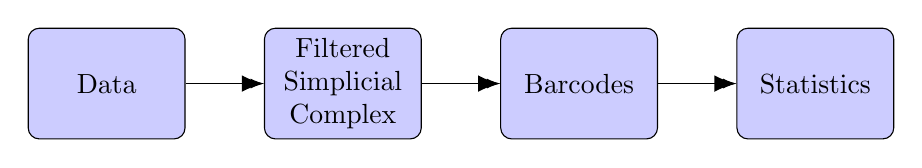
\begin{tikzpicture}[node distance = 2.5cm, auto, scale=0.8, decoration={
      markings,
      mark=at position 1 with {\arrow[scale=2,black]{latex}};
    }
  ]
   % Place nodes
    \node [block] (data) {Data};%Underling Probability Space
    \node [block, right of=data, node distance = 3cm] (simplex) {Filtered Simplicial Complex};
    \node [block, right of=simplex,node distance = 3cm] (pd) {Barcodes};
    \node [block, right of=pd, node distance = 3cm] (stat) {Statistics};
   % Draw edges
    \path [line, postaction={decorate}] (data) -- (simplex);
    \path [line, postaction={decorate}] (simplex) -- (pd);
    \path [line, postaction={decorate}] (pd) -- (stat);
  \end{tikzpicture}
\end{frame}

%------------------------------------------------------------------------

\begin{frame}
  \frametitle{Overview of PH}
\centering
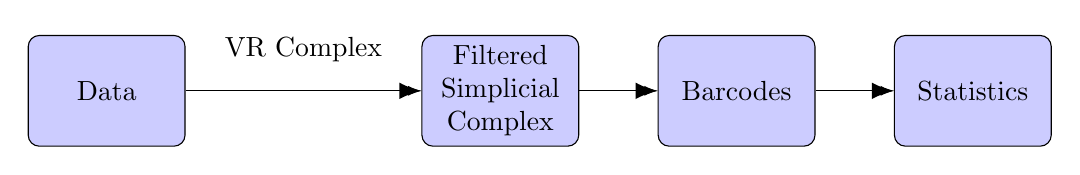
\begin{tikzpicture}[node distance = 2.5cm, auto, scale=0.8, decoration={
      markings, mark=at position 1 with {\arrow[scale=2,black]{latex}};
    }
  ]
   % Place nodes
    \node [block] (data) {Data};
    \node [block, right of=data, node distance = 5cm] (simplex) {Filtered Simplicial Complex};
    \node [block, right of=simplex,node distance = 3cm] (pd) {Barcodes};
    \node [block, right of=pd, node distance = 3cm] (stat) {Statistics};
   % Draw edges
    \path [line, postaction={decorate}] (data) -- (simplex) 
    node [midway, label=above:VR Complex] {};
    \path [line, postaction={decorate}] (simplex) -- (pd);
    \path [line, postaction={decorate}] (pd) -- (stat);
  \end{tikzpicture}
\end{frame}

%------------------------------------------------------------------------

\begin{frame}
  \frametitle{Simplicial Complexes from Point data}
  \only<1>{\begin{block}{Definition}
    A {\em point cloud} $P$ is a finite metric space.
  \end{block}
}
\only<2->{\begin{block}{Definition}
    The Vietoris-Rips complex is a simplicial complex built out of a point cloud. Put a circle
    of radius $r$ around each point. Add an edge whenever two circles overlap. 
    Add a triangle whenever three circles overlap.
\end{block}
}
  

  \begin{center}
    \only<+>{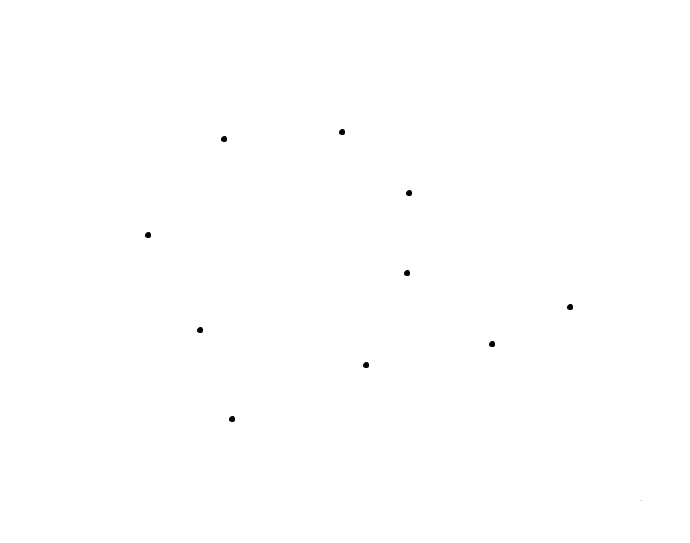
\includegraphics[trim=0 0 0 1cm, clip, scale=0.7]{images/VR_ex_r1.PNG}}
    \only<+>{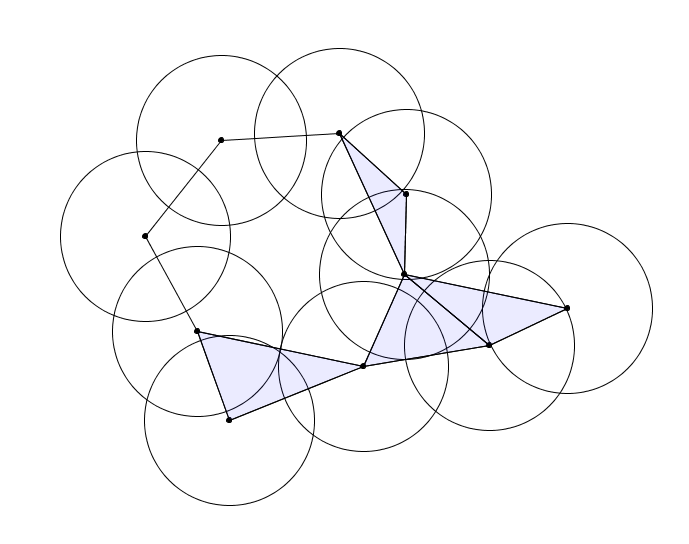
\includegraphics[trim=0 0 0 1cm, clip, scale=0.6]{images/VR_ex_r2.PNG}}
    \only<+>{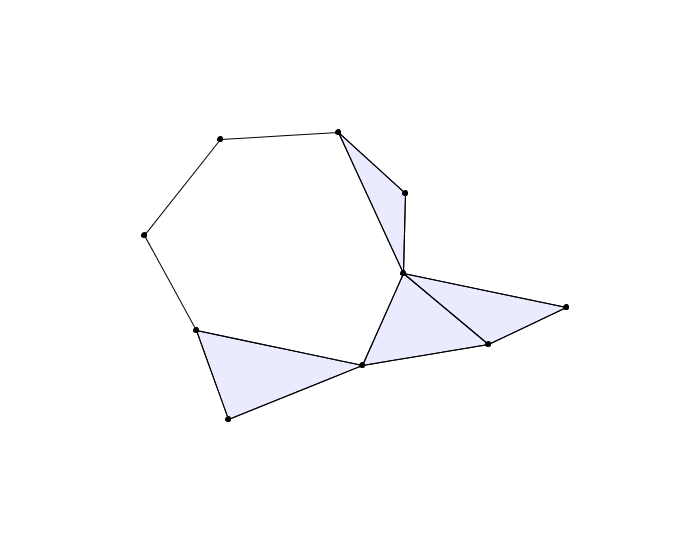
\includegraphics[trim=0 0 0 1cm, clip, scale=0.6]{images/VR_ex_r3.PNG}}
  \end{center}
\end{frame}

%------------------------------------------------------------------------

\begin{frame}{Vietoris-Rips parameter}
  \begin{block}{Question}
  How do we choose the correct radius for the Vietoris-Rips construction?
\end{block}

Often, there is no one ``right'' choice.
\begin{center}
  \only<+>{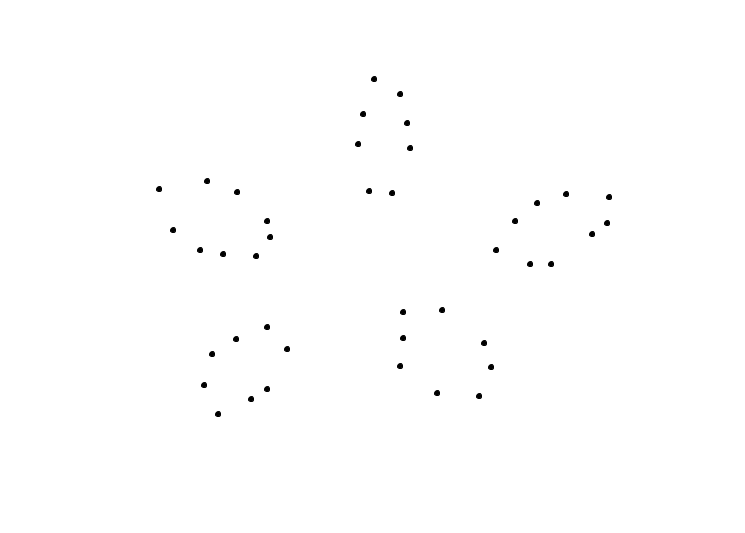
\includegraphics[trim= 0 0 0 1cm, clip, scale=0.7]{images/VR_ex_1.PNG}}
  \only<+>{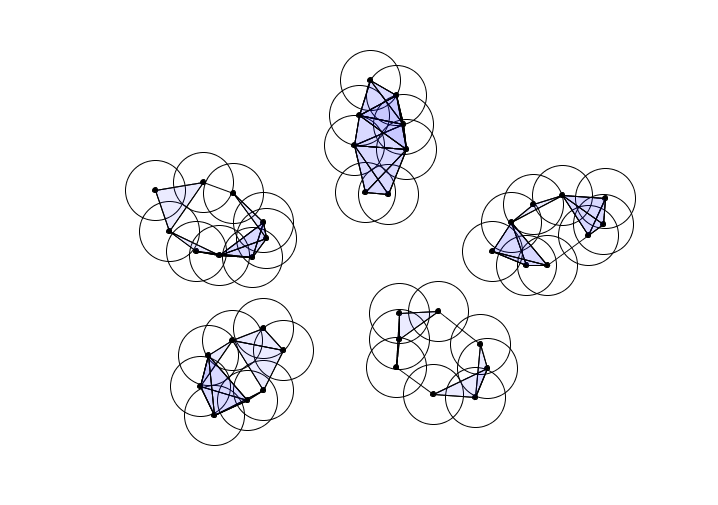
\includegraphics[trim= 0 0 0 1cm, clip, scale=0.7]{images/VR_ex_2.PNG}}
  \only<+>{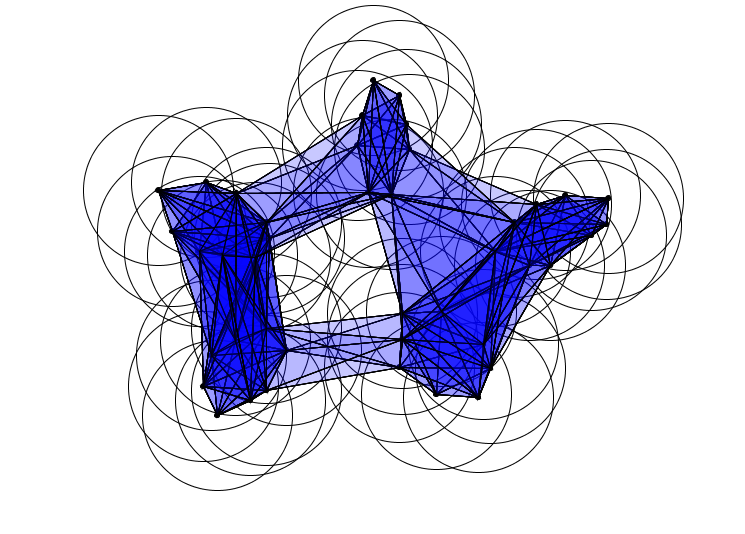
\includegraphics[trim= 0 0 0 1cm, clip, scale=0.7]{images/VR_ex_4.PNG}}
\end{center}
\end{frame}

%------------------------------------------------------------------------

\begin{frame}{Processing demo}
  \begin{center}
  Processing demo
\end{center}
\end{frame}

%------------------------------------------------------------------------

\begin{frame}{Overview of PH}
\centering
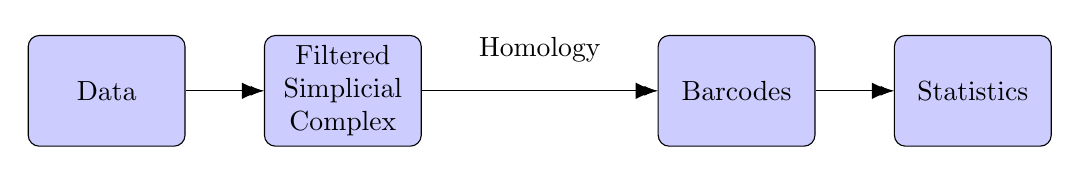
\begin{tikzpicture}[node distance = 2.5cm, auto, scale=0.8, decoration={
      markings,
      mark=at position 1 with {\arrow[scale=2,black]{latex}};
    }
  ]
   % Place nodes
    \node [block] (data) {Data};
    \node [block, right of=data, node distance = 3cm] (simplex) {Filtered Simplicial Complex};
    \node [block, right of=simplex,node distance = 5cm] (pd) {Barcodes};
    \node [block, right of=pd, node distance = 3cm] (stat) {Statistics};
   % Draw edges
    \path [line, postaction={decorate}] (data) -- (simplex);
    \path [line, postaction={decorate}] (simplex) -- (pd)
    node [midway, label=above:Homology] {};
    \path [line, postaction={decorate}] (pd) -- (stat);
  \end{tikzpicture}
\end{frame}

%------------------------------------------------------------------------

\begin{frame}{Barcodes}
  \begin{itemize}
    \item The barcode provides a summary of how the homology changes as the
      radius varies in the Vietoris-Rips construction.
    \item We look for topological features which `persist' over many values of radii.
  \end{itemize}

  Barcodes typically look like:

  \begin{minipage}{\textwidth}
  \begin{minipage}{0.5\textwidth}
    \centering
    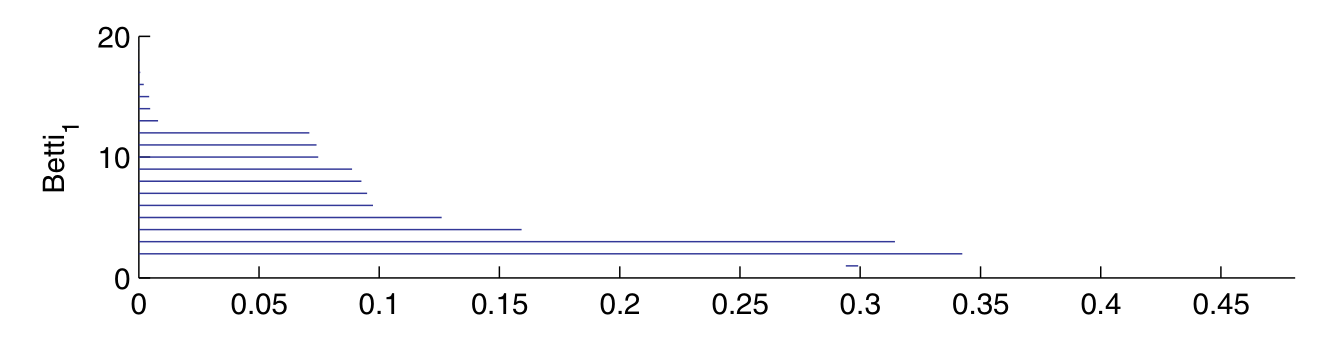
\includegraphics[scale=0.25]{images/betti1.png}
  \end{minipage}
  \begin{minipage}{0.5\textwidth}
    \centering
    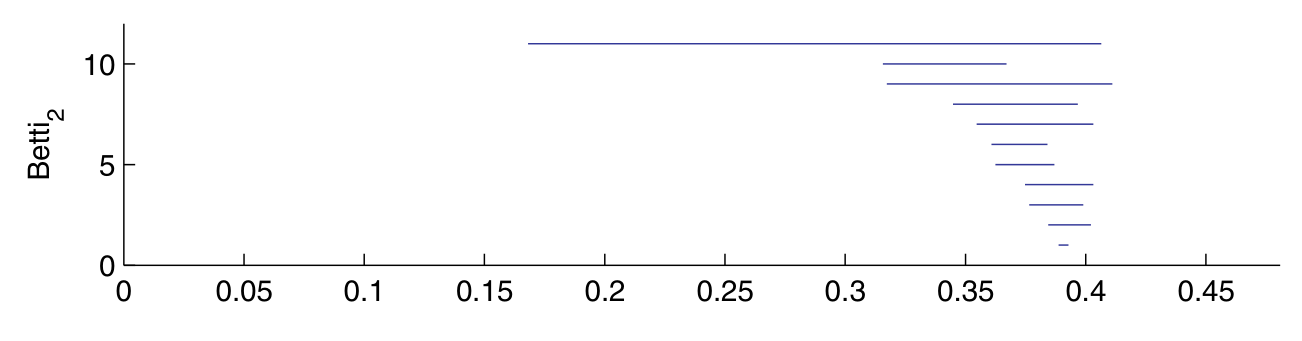
\includegraphics[scale=0.25]{images/betti2.png}
  \end{minipage}
\end{minipage}
\end{frame}
  
%==========================================================================

\section{JPDwB Tutorial}  
\begin{frame}{InteractiveJPDwB}
\begin{itemize}
\item Recall: Given a set of points $X$ and a parameter $r$, we can create a formal simplicial complex.
\item Let the $n$-simplex $\{x_0, x_1, \ldots, x_n\}$ exist if and only if $d(x_i, x_j) < r$ for all $0 \leq i,j\leq n$. 
\item We can visualize this process using InteractiveJPDwB.
\end{itemize}
\end{frame}

%-------------------------------------------------------------------------

\begin{frame}{InteractiveJPDwB}
\begin{itemize}
\item InteractiveJPDwB lets one visualize the generated simplicial complex for data in $\mathbb{R}^2$ and different values of $r$.
\item In other words, it demonstrates $0$-th and $1$-st degree persistence homology via barcodes.
\item Thanks to Michael Catanzaro, you can easily use this program on your own computer.
\item You can download this program from:
\begin{center}
\hyperref[https://github.com/MatthewZabka/LaberLabs18]{\textcolor{blue}{\texttt{https://github.com/MatthewZabka/LaberLabs18}}}
\end{center}
\end{itemize}
\end{frame}

%-----------------------------------------------------------------------------

\begin{frame}{Anwer the following!}
\begin{center}
\hyperref[https://github.com/MatthewZabka/LaberLabs18]{\textcolor{blue}{\texttt{https://github.com/MatthewZabka/LaberLabs18}}}
\end{center}
\begin{itemize}
\item What is the minimum number of points required so that $\beta_1 = 1$ for some value of $r$?
\item What is the minimum number of points required so that, for some $r$, we have $\beta_0 = 3$ and $\beta_1 = 2$?
\item What is the largest degree of homology that is geometrically feasible in $\mathbb{R}^2$?
\item What is the minimum number of points required to have $\beta_2 = 1$? In what dimension must the points lie?
\item What is the minimum number of points required to have $\beta_n = 1$?  In what dimension must the points lie?
\end{itemize}
\end{frame}

%-----------------------------------------------------------------------------

\begin{frame}{Group Discussion}
\begin{center}
{\Huge Discussion}
\end{center}
\begin{itemize}
\item What is the minimum number of points required so that $\beta_1 = 1$ for some value of $r$?
\item What is the minimum number of points required so that, for some $r$, we have $\beta_0 = 3$ and $\beta_1 = 2$?
\item What is the largest degree of homology that is geometrically feasible in $\mathbb{R}^2$?
\item What is the minimum number of points required to have $\beta_2 = 1$? In what dimension must the points lie?
\item What is the minimum number of points required to have $\beta_n = 1$?  In what dimension must the points lie?
\end{itemize}
\end{frame}

%========================================================================
\section{Persistence Homology and RIPSER}
%------------------------------------------------------------------------

\begin{frame}{Overview of Persistence Homology}
\centering
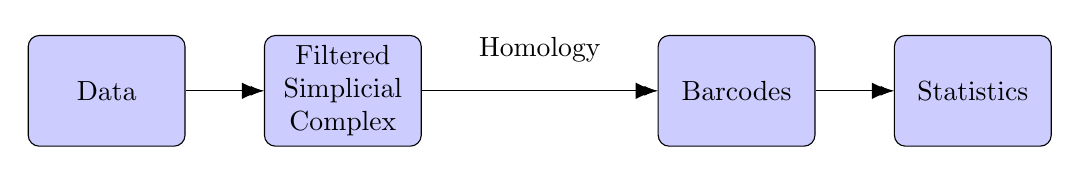
\begin{tikzpicture}[node distance = 2.5cm, auto, scale=0.8, decoration={
      markings,
      mark=at position 1 with {\arrow[scale=2,black]{latex}};
    }
  ]
   % Place nodes
    \node [block] (data) {Data};
    \node [block, right of=data, node distance = 3cm] (simplex) {Filtered Simplicial Complex};
    \node [block, right of=simplex,node distance = 5cm] (pd) {Barcodes};
    \node [block, right of=pd, node distance = 3cm] (stat) {Statistics};
   % Draw edges
    \path [line, postaction={decorate}] (data) -- (simplex);
    \path [line, postaction={decorate}] (simplex) -- (pd)
    node [midway, label=above:Homology] {};
    \path [line, postaction={decorate}] (pd) -- (stat);
  \end{tikzpicture}
\end{frame}

%------------------------------------------------------------------------

\begin{frame}{Barcodes}
  \begin{itemize}
    \item The barcode provides a summary of how the homology changes as the
      radius varies in the Vietoris-Rips construction.
    \item We look for topological features that `persist' over many values of radii.
  \end{itemize}

  Barcodes typically look like:

  \begin{minipage}{\textwidth}
  \begin{minipage}{0.5\textwidth}
    \centering
    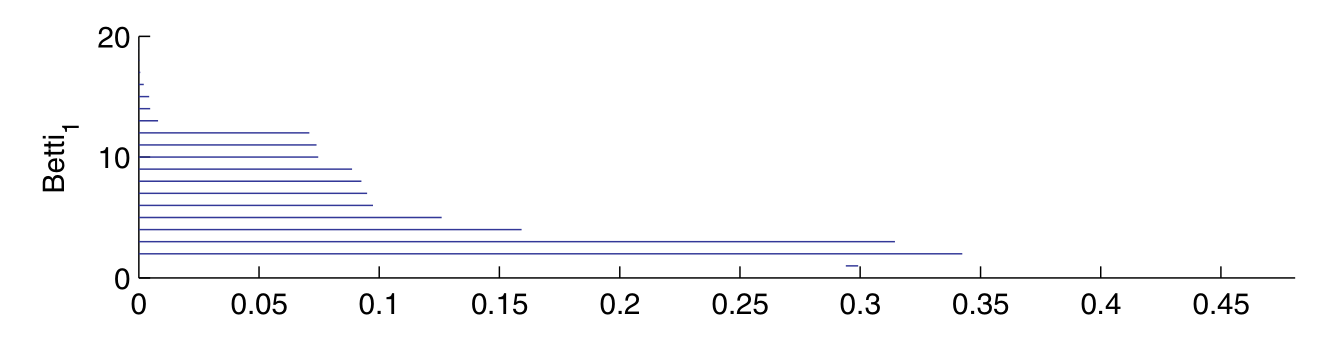
\includegraphics[scale=0.25]{images/betti1.png}
  \end{minipage}
  \begin{minipage}{0.5\textwidth}
    \centering
    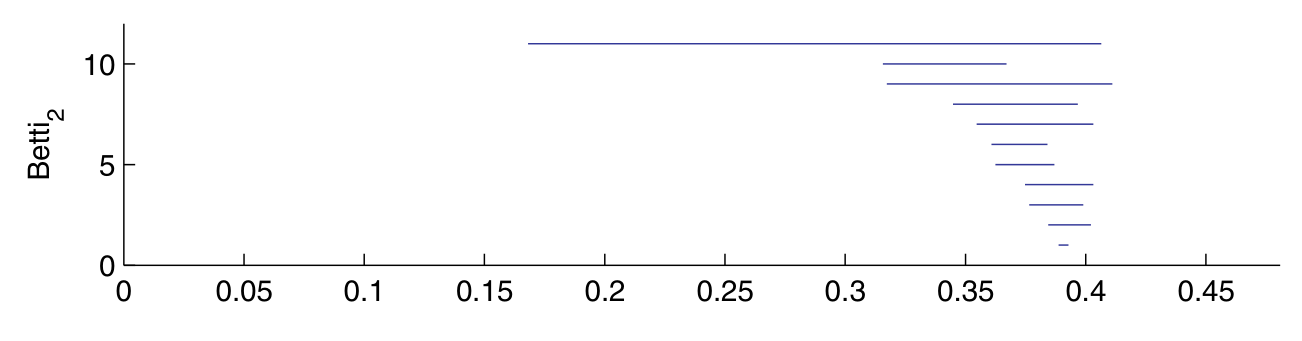
\includegraphics[scale=0.25]{images/betti2.png}
  \end{minipage}
\end{minipage}
\end{frame}
%----------------------------------------------------------------
\begin{frame}{Persistent Homology in Dimension 0 (Clustering)}
\begin{center}
\begin{tikzpicture}[scale = 1]
    \draw plot[mark=*, mark size = 0.5, only marks] file {data/clust1.txt};
    \draw plot[mark=*, mark size = 0.5, only marks] file {data/clust2.txt};
\end{tikzpicture}
\begin{itemize}
\item<1-> Start with a set of data in a metric space. Set $r=0$.
\item<2-> Increase $r$. Create an edge between two points whenever the distance between them is less than $r$. This creates a graph.
\item<3-> The graph defines a simplicial complex via Vietoris-Rips.
\item<4-> If a topological property (like a Betti number) \textit{persist} over a large range of $r$, we can conclude something about the structure of the data.
\item<5-> In this case, we should expect to see $\beta_0=2$ over a large range of $r$. 
\end{itemize}
\end{center}
\end{frame}
%--------------------------------------------------------
\begin{frame}{Persistent Homology in Dimension 0 (Clustering)}
\begin{center}
\begin{tikzpicture}[scale = 1]
    \draw plot[mark=*, mark size = 0.5] file {data/clust1.txt};
    \draw plot[mark=*, mark size = 0.5] file {data/clust2.txt};
\end{tikzpicture}
\end{center}
\begin{itemize}
\item<1-> A graph similar to this should persist over a large range of $r$.
\item<2-> How could we see the clusters if these data did not lie in $\mathbb{R}^2$?
\end{itemize}
\end{frame}
%-----------------------------------------------------
\begin{frame}{RIPSER}
\begin{itemize}
\item<1-> There are several programs that do persistence.
\item<2-> We shall first look at RIPSER.
\item<3-> Developed by Ulrich Bauer, RIPSER is a very fast C++ program for computing Vietoris-Rips persistence barcodes.
\item<4-> Let's try this on our data with two clusters.
\end{itemize}
\end{frame}
%-----------------------------------------------------
\begin{frame}{RIPSER}
\begin{center}
\begin{tikzpicture}[scale = 1]
    \draw plot[mark=*, mark size = 0.5, only marks] file {data/cloud1.txt};
\end{tikzpicture}
\end{center}
\begin{itemize}
\item<1-> You should already have these data -- stored as a \underline{point cloud}.
\begin{center}
\hyperref[https://github.com/MatthewZabka/LaberLabs18]{\textcolor{blue}{\texttt{https://github.com/MatthewZabka/LaberLabs18}}}
\end{center}
\item<2-> Input \texttt{cloud1.txt} into RIPSER:
\begin{center}
\hyperref[https://live.ripser.org/]{\textcolor{blue}{\texttt{https://live.ripser.org/}}}
\end{center}
\end{itemize}
\end{frame}
%------------------------------------------------------
\begin{frame}{Persistent Homology}
\begin{itemize}
\item<1-> Suppose we have data that lie on the circle.
\begin{center}
\begin{figure}
\begin{tikzpicture}[scale = 1.5]
    \draw plot[mark=*, mark size = 0.5, only marks] file {data/cloud2.txt};
\end{tikzpicture}
\caption{An unrealistic example \texttt{cloud2.txt}, where data lie perfectly on $S^1$.}
\end{figure}
\end{center}
\item<2-> Input \texttt{cloud2.txt} into RIPSER.
\end{itemize}
\end{frame}
%------------------------------------------------------
\begin{frame}{Persistent Homology}
\begin{itemize}
\item<1-> Suppose we have data that \textbf{almost} lie on the circle.
\begin{center}
\begin{figure}
\begin{tikzpicture}[scale = 1.5]
    \draw plot[mark=*, mark size = 0.5, only marks] file {data/cloud3.txt};
\end{tikzpicture}
\caption{A slightly more realistic example \texttt{cloud3.txt}.}
\end{figure}
\end{center}
\item<2-> We want to analyze data we cannot see!
\end{itemize}
\end{frame}
%------------------------------------------------------
\begin{frame}{Persistent Homology}
\begin{center}
\hyperref[https://github.com/MatthewZabka/LaberLabs18]{\textcolor{blue}{\texttt{https://github.com/MatthewZabka/LaberLabs18}}}
\end{center}
\begin{itemize}
\item Now it is your turn! Data are located in the \texttt{RIPSERdata} folder that you have already downloaded!
\item Input \texttt{cloud1.txt} int RIPSER. Confirm that two generators of $H_0$ persist. (i.e. $\beta_0 = 2$)
\item Input \texttt{cloud2.txt} into RIPSER. Confirm that one generator for $H_0$ and one generator for $H_1$ persist. (i.e. $\beta_0 = 1$ and $\beta_1 = 1$)
\item Input \texttt{cloud3.txt} into RIPSER. Confirm that one generator for $H_0$ and one generator for $H_1$ persist. (i.e. $\beta_0 = 1$ and $\beta_1 = 1$)
\item Try inputting \texttt{cloud4.txt} into RIPSER up to distance 2. What can you say about the data's shape?
\item Try some actual data! \texttt{cloud5.txt} (Test up to distance 150.)
\item More actual data! \texttt{cloud6.txt} (Test up to distance 2.)
\end{itemize}
\end{frame}
%------------------------------------------------------
\begin{frame}{Persistent Homology}
\begin{center}
{\Huge Discussion}
\end{center}
\begin{itemize}
\item What is the shape of \texttt{cloud4.txt}?
\item What is the shape of \texttt{cloud5.txt}?
\item What is the shape of \texttt{cloud6.txt}?
\end{itemize}

\end{frame}
%------------------------------------------------------
\begin{frame}{Combining Persistence and Other Methods}
\begin{itemize}
\item Suppose we had a barcode in dimension 1 that looked as follows:
\begin{figure}
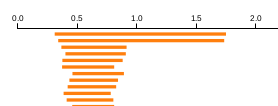
\includegraphics[scale=0.5]{images/torusbar.png}
\end{figure}
\item What are are possibilities for the manifold on which the data lie?
\end{itemize}
\end{frame}
%-------------------------------------
\begin{frame}{Combining Persistence and Other Methods}
\begin{itemize}
\item Suppose we had a barcode in dimension 1 that looked as follows:
\begin{figure}
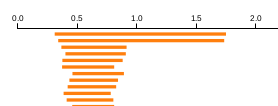
\includegraphics[scale=0.5]{images/torusbar.png}
\end{figure}
\item Suppose we perform PCA and get the following projection:
\begin{figure}
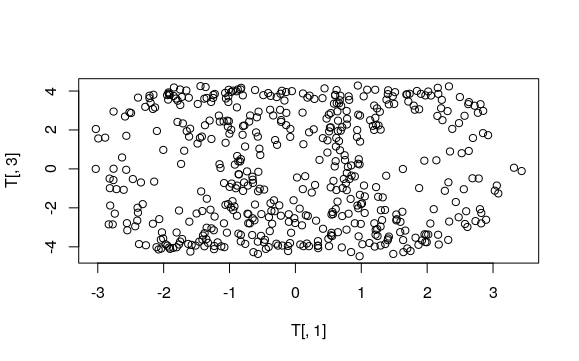
\includegraphics[scale=0.3]{images/torusPCA.png}
\end{figure}
\item What does PCA suggest about the dimension of the manifold? 
\item What does this suggest about the space on which the data lie?
\end{itemize}
\end{frame}

%=======================================================================

\section{Multiparameter Persistence and RIVET}
\begin{frame}{RIVET}
\begin{itemize}
\item<1-> Let's think about how this could go wrong and how we could fix it!
\item<2-> Suppose that, instead of data that look like this:
\begin{figure}
\begin{tikzpicture}[scale = 1.5]
    \draw plot[mark=*, mark size = 0.5, only marks] file {data/cloud3.txt};
\end{tikzpicture}
\end{figure} 
\end{itemize}
\end{frame}

%---------------------------------------------------------------

\begin{frame}{RIVET}
\begin{itemize}
\item Let's think about how this could go wrong and how we could fix it!
\item We had data that looked like this:
\begin{figure}
\begin{tikzpicture}[scale = 0.5]
    \draw plot[mark=*, mark size = 1.5, only marks] file {data/data7.txt};
\end{tikzpicture}
\end{figure} 
\end{itemize}
\end{frame}

%---------------------------------------------------------------

\begin{frame}{RIVET}
\begin{itemize}
\item<1-> This is a much more realistic example.
\item<2-> The blue points -- noise -- will make it hard to see the generator of $H_1$.
\begin{figure}
\begin{tikzpicture}[scale = 0.5]
    \draw plot[mark=*, mark size = 1.5, only marks] file {data/data7.txt};
    \draw[color = blue] plot[mark=*, mark size = 1.5, only marks] file {data/data7noise.txt};
\end{tikzpicture}
\end{figure} 
\end{itemize}
\end{frame}

%---------------------------------------------------------------

\begin{frame}{RIVET}
The first barcode includes the entire data set.  The second barcode eliminates the blue 'noise'.

\begin{figure}
\centering
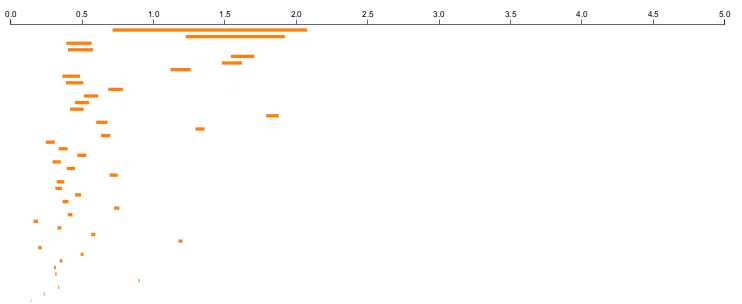
\includegraphics[scale=0.35]{images/data7.png}
\end{figure} 

\begin{figure}
\centering
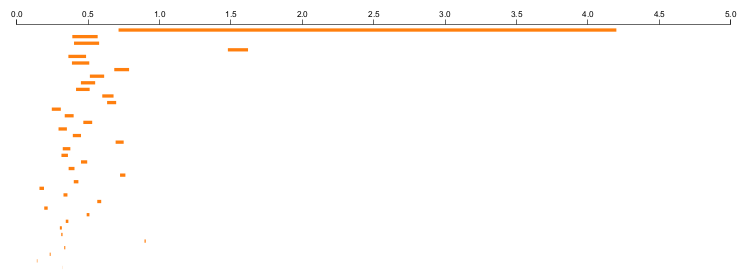
\includegraphics[scale=0.35]{images/data7nonoise.png}
\end{figure} 
\end{frame}

%---------------------------------------------------------------

\begin{frame}{RIVET}
\begin{itemize}
\item<1-> One way to deal with such situations: consider the density of the points.
\begin{figure}
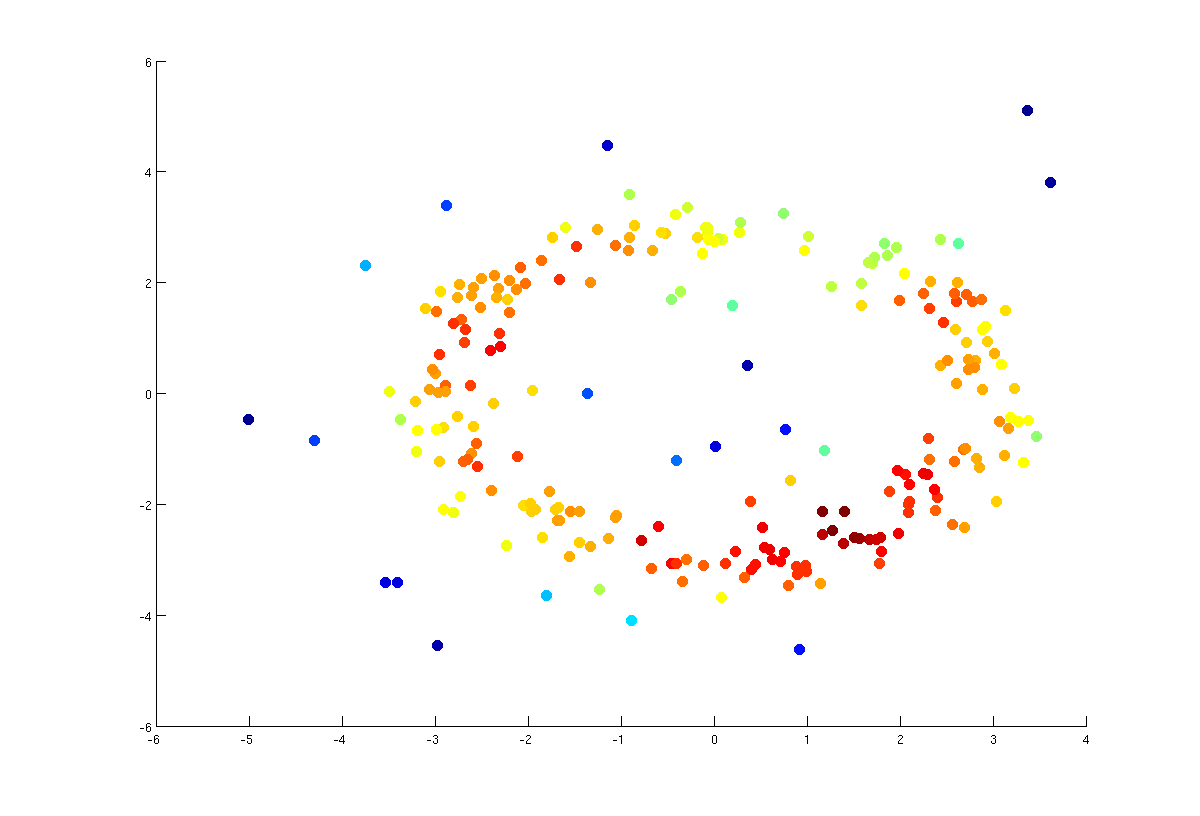
\includegraphics[scale=0.2]{images/data7density}
\caption{A density heat map of the data}
\end{figure} 
\item<2-> Letting the density threshold vary results in \textbf{multi-parameter persistence}!
\end{itemize}
\end{frame}

%---------------------------------------------------------------

\begin{frame}{RIVET}
\begin{itemize}
\item Michael Lesnick and Matthew Wright have written a program for visualizing multiparameter persistence.
\item Installation is not so simple.
\item Let us try to use RIVET on this example together.
\end{itemize}
\end{frame}

%---------------------------------------------------------------

\begin{frame}{RIVET}
\begin{center}
{\Huge Thank you!}\\

\href{mailto:matthew.zabka@smsu.edu}{\textcolor{blue}{matthew.zabka@smsu.edu}}
\end{center}
\end{frame}

%=========================================================================
%==========================================================================

\begin{frame}{References}
\nocite{ghrist2017homological, bubenik_statistical_2015, carlsson_topology_2009,
oudot2015persistence, perea_brief_2018, wright}

\renewcommand*{\bibfont}{\small}
General Overviews:
\printbibliography[keyword=intro]

More technical introduction:
\printbibliography[keyword=nintro]

\end{frame}
%----------------------------------------------------------------------
\begin{frame}{References}
\nocite{Wolcott2016InteractiveJPDwB, bauer2017ripser, lesnick2015interactive}

Software
\printbibliography[keyword=software]
\end{frame}


\end{document}
